
% Programming/Coding Assignment
% LaTeX Template
%
% This template has been downloaded from:
% http://www.latextemplates.com
%
% Original author:
% Ted Pavlic (http://www.tedpavlic.com)
%
% Note:
% The \lipsum[#] commands throughout this template generate dummy text
% to fill the template out. These commands should all be removed when 
% writing assignment content.
%
% This template uses a Perl script as an example snippet of code, most other
% languages are also usable. Configure them in the "CODE INCLUSION 
% CONFIGURATION" section.
%
%%%%%%%%%%%%%%%%%%%%%%%%%%%%%%%%%%%%%%%%%

%----------------------------------------------------------------------------------------
%   PACKAGES AND OTHER DOCUMENT CONFIGURATIONS
%----------------------------------------------------------------------------------------

\documentclass{article}

\usepackage{fancyhdr} % Required for custom headers
\usepackage{lastpage} % Required to determine the last page for the footer
\usepackage{extramarks} % Required for headers and footers
\usepackage[usenames,dvipsnames]{color} % Required for custom colors
\usepackage{graphicx} % Required to insert images
\usepackage{listings} % Required for insertion of code
\usepackage{courier} % Required for the courier font
\usepackage{lipsum} % Used for inserting dummy 'Lorem ipsum' text into the template
\usepackage{fullpage,amsthm,amsfonts,amssymb,epsfig,amsmath}

% Margins
\topmargin=-0.45in
\evensidemargin=0in
\oddsidemargin=0in
\textwidth=6.5in
\textheight=9.0in
\headsep=0.25in

\linespread{1.1} % Line spacing

% Set up the header and footer
\pagestyle{fancy}
\lhead{\hmwkAuthorName} % Top left header
\chead{\hmwkClass\ (\hmwkClassInstructor\ \hmwkClassTime): \hmwkTitle} % Top center head
\rhead{\firstxmark} % Top right header
\lfoot{\lastxmark} % Bottom left footer
\cfoot{} % Bottom center footer
\rfoot{Page\ \thepage\ of\ \protect\pageref{LastPage}} % Bottom right footer
\renewcommand\headrulewidth{0.4pt} % Size of the header rule
\renewcommand\footrulewidth{0.4pt} % Size of the footer rule
\newcommand{\tab}{\hspace*{3em}}

\setlength\parindent{0pt} % Removes all indentation from paragraphs

%----------------------------------------------------------------------------------------
%   CODE INCLUSION CONFIGURATION
%----------------------------------------------------------------------------------------

\definecolor{MyDarkGreen}{rgb}{0.0,0.4,0.0} % This is the color used for comments
\lstloadlanguages{Perl} % Load Perl syntax for listings, for a list of other languages supported see: ftp://ftp.tex.ac.uk/tex-archive/macros/latex/contrib/listings/listings.pdf
\lstset{language=Perl, % Use Perl in this example
        frame=single, % Single frame around code
        basicstyle=\small\ttfamily, % Use small true type font
        keywordstyle=[1]\color{Blue}\bf, % Perl functions bold and blue
        keywordstyle=[2]\color{Purple}, % Perl function arguments purple
        keywordstyle=[3]\color{Blue}\underbar, % Custom functions underlined and blue
        identifierstyle=, % Nothing special about identifiers                                         
        commentstyle=\usefont{T1}{pcr}{m}{sl}\color{MyDarkGreen}\small, % Comments small dark green courier font
        stringstyle=\color{Purple}, % Strings are purple
        showstringspaces=false, % Don't put marks in string spaces
        tabsize=5, % 5 spaces per tab
        %
        % Put standard Perl functions not included in the default language here
        morekeywords={rand},
        %
        % Put Perl function parameters here
        morekeywords=[2]{on, off, interp},
        %
        % Put user defined functions here
        morekeywords=[3]{test},
        %
        morecomment=[l][\color{Blue}]{...}, % Line continuation (...) like blue comment
        numbers=left, % Line numbers on left
        firstnumber=1, % Line numbers start with line 1
        numberstyle=\tiny\color{Blue}, % Line numbers are blue and small
        stepnumber=5 % Line numbers go in steps of 5
}

% Creates a new command to include a perl script, the first parameter is the filename of the script (without .pl), the second parameter is the caption
\newcommand{\perlscript}[2]{
\begin{itemize}
\item[]\lstinputlisting[caption=#2,label=#1]{#1.pl}
\end{itemize}
}

%----------------------------------------------------------------------------------------
%   DOCUMENT STRUCTURE COMMANDS
%   Skip this unless you know what you're doing
%----------------------------------------------------------------------------------------

% Header and footer for when a page split occurs within a problem environment
\newcommand{\enterProblemHeader}[1]{
\nobreak\extramarks{#1}{#1 continued on next page\ldots}\nobreak
\nobreak\extramarks{#1 (continued)}{#1 continued on next page\ldots}\nobreak
}

% Header and footer for when a page split occurs between problem environments
\newcommand{\exitProblemHeader}[1]{
\nobreak\extramarks{#1 (continued)}{#1 continued on next page\ldots}\nobreak
\nobreak\extramarks{#1}{}\nobreak
}

\setcounter{secnumdepth}{0} % Removes default section numbers
\newcounter{homeworkProblemCounter} % Creates a counter to keep track of the number of problems

\newcommand{\homeworkProblemName}{}
\newenvironment{homeworkProblem}[1][Problem \arabic{homeworkProblemCounter}]{ % Makes a new environment called homeworkProblem which takes 1 argument (custom name) but the default is "Problem #"
\stepcounter{homeworkProblemCounter} % Increase counter for number of problems
\renewcommand{\homeworkProblemName}{#1} % Assign \homeworkProblemName the name of the problem
\section{\homeworkProblemName} % Make a section in the document with the custom problem count
\enterProblemHeader{\homeworkProblemName} % Header and footer within the environment
}{
\exitProblemHeader{\homeworkProblemName} % Header and footer after the environment
}

\newcommand{\problemAnswer}[1]{ % Defines the problem answer command with the content as the only argument
\noindent\framebox[\columnwidth][c]{\begin{minipage}{0.98\columnwidth}#1\end{minipage}} % Makes the box around the problem answer and puts the content inside
}

\newcommand{\homeworkSectionName}{}
\newenvironment{homeworkSection}[1]{ % New environment for sections within homework problems, takes 1 argument - the name of the section
\renewcommand{\homeworkSectionName}{#1} % Assign \homeworkSectionName to the name of the section from the environment argument
\subsection{\homeworkSectionName} % Make a subsection with the custom name of the subsection
\enterProblemHeader{\homeworkProblemName} % Header and footer within the environment
}{
\enterProblemHeader{\homeworkProblemName} % Header and footer after the environment
}

%----------------------------------------------------------------------------------------
%   NAME AND CLASS SECTION
%----------------------------------------------------------------------------------------

\newcommand{\hmwkTitle}{Homework\ \#5} % Assignment title
\newcommand{\hmwkDueDate}{Tuesday,\ May\ 12st,\ 2015} % Due date
\newcommand{\hmwkClass}{CMPS\ 102} % Course/class
\newcommand{\hmwkClassTime}{4:00pm} % Class/lecture time
\newcommand{\hmwkClassInstructor}{Warmuth} % Teacher/lecturer
\newcommand{\hmwkAuthorName}{John Allard \ 1437547
} % Your name


%----------------------------------------------------------------------------------------
%----------------------------------------------------------------------------------------
%   USER SETTINGS
%----------------------------------------------------------------------------------------
%----------------------------------------------------------------------------------------
\usepackage{mathtools}
\DeclarePairedDelimiter\ceil{\lceil}{\rceil}
\DeclarePairedDelimiter\floor{\lfloor}{\rfloor}



%----------------------------------------------------------------------------------------
%   TITLE PAGE
%----------------------------------------------------------------------------------------

\title{
\vspace{2in}
\textmd{\textbf{\hmwkClass:\ \hmwkTitle}}\\
\normalsize\vspace{0.1in}\small{Due\ on\ \hmwkDueDate}\\
\vspace{0.1in}\large{\textit{}}
\vspace{3in}
}

\author{\textbf{\hmwkAuthorName}}
\date{} % Insert date here if you want it to appear below your name

%----------------------------------------------------------------------------------------

\begin{document}

\maketitle

%----------------------------------------------------------------------------------------
%   TABLE OF CONTENTS
%----------------------------------------------------------------------------------------

%\setcounter{tocdepth}{1} % Uncomment this line if you don't want subsections listed in the ToC

% \tableofcontents
\newpage





%----------------------------------------------------------------------------------------
%   PROBLEM 1
%----------------------------------------------------------------------------------------

% To have just one problem per page, simply put a \clearpage after each problem

\begin{homeworkProblem}

\noindent A rabbit wants to go through a distance of n feet. It can either do a short hop of one foot or a long hop of three feet. Denote f(n) as the number of ways that the rabbit can go through a distance of n feet. 

\noindent Give an O(n) algorithm to find f(n).

\begin{enumerate}

\item a.) For a given $n \geq 0$, $f(n)$ depends directly on $f(n-1)$ and $f(n-3)$. This is because the only ways to get to $n$ under the rules of our game are to either jump from $n-1$ or $n-3$. 

\item b.) The subproblems are related additively, in that the solution to a problem of size $n$ is the sum of the solutions to problems of size $n-1$ and $n-3$. This is because, as stated above, these two subproblems are the only ones that can lead to a problem of size $n$. Combine that with the fact that $n-1$ and $n-3$ are always different numbers, than their solution values must be different (they are different locations so the paths taken to go them must be different from one another), so we can simply add the value of $f(n-1)$ and $f(n-3)$ to get $f(n)$.

\item c.) $ \forall n \geq 0$ : $ f(n) = f(n-1) + f(n-3)$ : $f(0) = 1$ \\ The base case might seem weird but it makes the recursion work. I could have also defined $f(1)$ and $f(3)$, but this way seemed easier. This recursion leads to an unbalanced tree, and to get solution to $f(n)$ you can simply count the leaves. Intuitively this corresponds to a unique path being traced back from $n$ to $0$, the starting point for the rabbit. At each subproblem, we have only two ways to go, trace ourselves back a single foot or a 3-foot step. Since these two values are unique, any paths that lead to them are also unique, and thus they should be added to get the value for the current subproblem. 

\item d.) Since this problem is one dimensionsal (over $n$), we only need an array of length $n$ to perform memoization. Everytime $f(n)$ is called, we see is the array index at position $n$ is empty, if so we perform our calculation by continuing the recursion and enter it into the table once we find the value, if it is not empty we simply extract the value from the array in constant time, bottoming out the recursion early. \\

\item e.) Two arrows would be pointing out from $n$ backwards along a single axis, one landing on $n-1$ and the other landing on $n-3$.

\item f.) // Give proof of algorithms correctness and run-time here, shouldn't be too difficult.

The algorithm is given below \\

\begin{lstlisting}
// M = memoization array of length n, starts empty
// n > 0 is the f(n) value we are querying
findpaths(n,M) :
  M[0] = 0
  for i in [1 ... n] // inclusive of ends
    if i < 3 : // make sure we do not index negatives
      M[i] = M[i-1]
    else :
      M[i] = M[i-1]+M[i-3]

  return M[n] 
\end{lstlisting}

\end{enumerate}


\end{homeworkProblem}






%----------------------------------------------------------------------------------------
%   PROBLEM 2
%----------------------------------------------------------------------------------------

\begin{homeworkProblem}

\vspace{2mm}

Let $G = (V, E)$ be an undirected graph with $n$ nodes.  Recall that a subset of the nodes is called an independent set if no two of them are joined by an edge. Finding large independent sets is difficult in general; but here we'll see that it can be done efficiently if the graph is ``simple'' enough. 

Call a graph $G = (V, E)$ a path if its nodes can be written as $v_1, v_2, ...,v_n$, with an edge between vi and $v_j$ if and only if the numbers $i$ and $j$ differ by exactly 1. With each node $v_i$, we associate a positive integer weight $w_i$. 

Consider, for example, the five-node path drawn in Figure 6.28. The weights are the numbers drawn inside the nodes. 

The goal in this question is to solve the following problem:

\vspace{2mm}

\emph{Find an independent set in a path G whose total weight is as large as possible.}

\vspace{2mm}

\noindent \textbf{(a)} Give an example to show that the following algorithm does not always find an independent set of maximum total weight.

\begin{lstlisting}
The "heaviest-first" greedy algorithm 
  Start with S equal to the empty set 
  While some node remains in G 
    Pick a node vi of maximum weight 
    Add vi to S 
    Delete vi and its neighbors from G 
  Endwhile 
  Return S
\end{lstlisting}

\noindent \textbf{(b)} Give an example to show that the following algorithm also does not always find an independent set of maximum total weight.

\begin{lstlisting}
Let S1 be the set of all vi where i is an odd number 
Let S2 be the set of all vi where i is an even number 
(Note that S1 and S2 are both independent sets) Determine which of S1 or S2 has greater total weight, and return this one

\end{lstlisting}

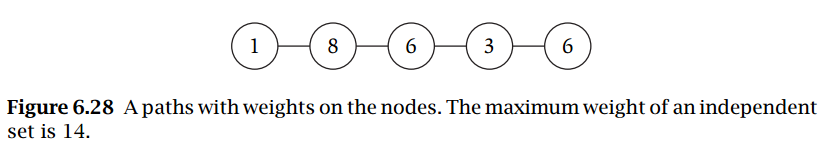
\includegraphics[scale=0.75]{1.PNG}

\vspace{2mm}

\noindent \textbf{(c)}  Give an algorithm that takes an n-node path G with weights and returns an independent set of maximum total weight. The running time should be polynomial in n, independent of the values of the weights.

\vspace{6mm}

\end{homeworkProblem}





%----------------------------------------------------------------------------------------
%   PROBLEM 3
%----------------------------------------------------------------------------------------
\begin{homeworkProblem}

\vspace{2mm}

\noindent Let $G = (V, E)$ be a directed graph with nodes $v_1, ..., v_n$. We say that G is an ordered graph if it has the following properties. 

\vspace{2mm}

\textbf{(i)} Each edge goes from a node with a lower index to a node with a higher index. That is, every directed edge has the form $(v_i, v_j)$ with $i < j$. 

\vspace{2mm}

\textbf{(ii)} Each node except vn has at least one edge leaving it. That is, for every node $v_i$, $i = 1, 2, ..., n − 1$, there is at least one edge of the form $(v_i,v_j)$. 

\vspace{2mm}

The length of a path is the number of edges in it. The goal in this question is to solve the following problem (see Figure 6.29 for an example).

\vspace{2mm}

\emph{Given an ordered graph G, find the length of the longest path that begins at $v_1$ and ends at $v_n$.}

\vspace{2mm}

\noindent \textbf{(a)} Show that the following algorithm does not correctly solve this problem, by giving an example of an ordered graph on which it does not return the correct answer.

\begin{lstlisting}
Set w = v_1
Set L = 0

While there is an edge out of the node w 
  Choose the edge (w, v_j) 
    for which j is as small as possible 
  Set w = v_j   
  Increase L by 1 
end while 
Return L as the length of the longest path

\end{lstlisting}

\vspace{2mm}

In your example, say what the correct answer is and also what the algorithm above finds.

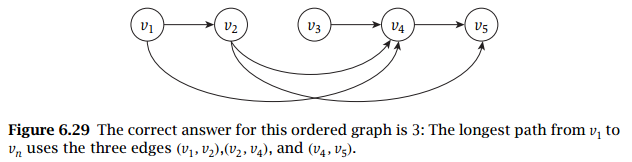
\includegraphics[scale=1]{2.PNG}

\vspace{2mm}

\noindent \textbf{(b)} Give an efficient algorithm that takes an ordered graph G and returns  the length of the longest path that begins at $v_1$ and ends at $v_n$.(Again, the length of a path is the number of edges in the path.)

\vspace{6mm}

\end{homeworkProblem}





%----------------------------------------------------------------------------------------
%   PROBLEM 4
%----------------------------------------------------------------------------------------
\begin{homeworkProblem}


\vspace{2mm}

\noindent In a word processor, the goal of ``pretty-printing'' is to take text with a ragged right margin, like this,

\vspace{2mm}

\begin{lstlisting}
Call me Ishmael. 
Some years ago, 
never mind how long precisely,
having little or no money in my purse, 
and nothing particular to interest me on shore, 
I thought I would sail about a little 
and see the watery part of the world.

\end{lstlisting}

\vspace{2mm}

\noindent and turn it into text whose right margin is as ``even'' as possible, like this.

\vspace{2mm}

\begin{lstlisting}

Call me Ishmael. Some years ago, never 
mind how long precisely, having little 
or no money in my purse, and nothing 
particular to interest me on shore, I 
thought I would sail about a little 
and see the watery part of the world.

\end{lstlisting}

\vspace{2mm}

To make this precise enough for us to start thinking about how to write a pretty-printer for text, we need to figure out what it means for the right margins to be ``even.'' So suppose our text consists of a sequence of words, $W={w_1,w_2,...,w_n}$, where $w_i$ consists of $c_i$ characters. We have a maximum line length of L. We will assume we have a fixed-width font and ignore issues of punctuation or hyphenation. 

A formatting of W consists of a partition of the words in W into lines. In the words assigned to a single line, there should be a space after each word except the last; and so if $w_j, w_{j+1}, ..., w_k$ are assigned to one line, then we should have 

\centerline{ $\displaystyle[\sum_{i = j}^{k - 1} (c_i + 1)] + c_k \le L.$
}

\noindent We will call an assignment of words to a line valid if it satisfies this inequality. The difference between the left-hand side and the right-hand side will be called the slack of the line—that is, the number of spaces left at the right margin. 

Give an efficient algorithm to find a partition of a set of words W into valid lines, so that the sum of the squares of the slacks of all lines (including the last line) is minimized.

\vspace{6mm}


\end{homeworkProblem}






%----------------------------------------------------------------------------------------
%   PROBLEM 5
%----------------------------------------------------------------------------------------
\begin{homeworkProblem}


\vspace{2mm}

\emph{Gerrymandering} is the practice of carving up electoral districts in very careful ways so as to lead to outcomes that favor a particular political party. Recent court challenges to the practice have argued that through this calculated redistricting, large numbers of voters are being effectively (and intentionally) disenfranchised. 

Computers, it turns out, have been implicated as the source of some of the ``villainy'' in the news coverage on this topic: Thanks to powerful software, gerrymandering has changed from an activity carried out by a bunch of people with maps,pencil,and paper into the industrial-strength process that it is today. Why is gerrymandering a computational problem? There are database issues involved in tracking voter demographics down to the level of individual streets and houses; and there are algorithmic issues involved in grouping voters into districts. Let's think a bit about what these latter issues look like. 

Suppose we have a set of n precincts $P1, P2, ..., Pn$, each containing m registered voters. We're supposed to divide these precincts into two districts, each consisting of $n/2$ of the precincts. Now, for each precinct, we have information on how many voters are registered to each of two political parties. (Suppose, for simplicity, that every voter is registered to one of these two.) We'll say that the set of precincts is susceptible to gerrymandering if it is possible to perform the division into two districts in such a way that the same party holds a majority in both districts.

Give an algorithm to determine whether a given set of precincts is susceptible to gerrymandering; the running time of your algorithm should be polynomial in $n$ and $m$. 

\vspace{2mm}

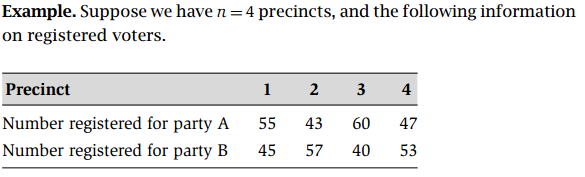
\includegraphics[scale=0.75]{3.PNG}

\vspace{2mm}

This set of precincts is susceptible since, if we grouped precincts 1 and 4 into one district, and precincts 2 and 3 into the other, then party A would have a majority in both districts. (Presumably, the ``we'' who are doing the grouping here are members of party A.) This example is a quick illustration of the basic unfairness in gerrymandering: Although party A holds only a slim majority in the overall population (205 to 195), it ends up with a majority in not one but both districts.

\vspace{6mm}


\end{homeworkProblem}






%----------------------------------------------------------------------------------------
%   PROBLEM 6
%----------------------------------------------------------------------------------------
\begin{homeworkProblem}


\vspace{2mm}

Recall the scheduling problem from Section 4.2 in which we sought to minimize the maximum lateness. There are $n$ jobs, each with a deadline $d_i$ and a required processing time $t_i$, and all jobs are available to be scheduled starting at time $s$. For a job $i$ to be done, it needs to be assigned a period from $s_i \ge s$ to $f_i = s_i + t_i$, and different jobs should be assigned nonoverlapping intervals. As usual, such an assignment of times will be called a schedule. 

In this problem, we consider the same setup, but want to optimize a different objective. In particular, we consider the case in which each job must either be done by its deadline or not at all. We'll say that a subset J of the jobs is schedulable if there is a schedule for the jobs in J so that each of them finishes by its deadline. Your problem is to select a schedulable subset of maximum possible size and give a schedule for this subset that allows each job to finish by its deadline. 

\vspace{2mm}

\noindent \textbf{(a)} Prove that there is an optimal solution $J$ (i.e., a schedulable set of maximum size) in which the jobs in $J$ are scheduled in increasing order of their deadlines. 

\vspace{2mm}

\noindent \textbf{(b)} Assume that all deadlines $d_i$ and required times $t_i$ are integers. Give an algorithm to find an optimal solution. Your algorithm should run in time polynomial in the number of jobs $n$, and the maximum deadline $D = max_i d_i$. 


\end{homeworkProblem}



%----------------------------------------------------------------------------------------

\end{document}